\chapter[Aplicando Minería de Datos con RapidMiner]{Aplicando Minería de Datos con RapidMiner}
\label{ch:desmin}

\section{Identificación de datos y variables}
\subsection{Recolección de Datos}

Los datos a utilizar en los modelos a presentar en este capítulo son extraídos de la base de datos de una institución privada. Estos datos corresponden a información de los años 2014 y 2015 de alumnos de las distintas carreras de ingeniería que imparte la institución. Además, se extrae información a través del SIES sobre la institución y sus diferentes carreras de ingeniería con respecto a acreditación e índices de empleabilidad.\\

Los datos proporcionados por la institución se encuentran en un archivo Excel en el cual figuran los siguientes datos: Rut del estudiante, Apellido paterno del estudiante, Apellido materno del estudiante, Nombres del estudiante, Comuna de residencia del estudiante, Ciudad de residencia del estudiante, Facultad del estudiante, Carrera del estudiante, Jornada del estudiante, PSU de lenguaje, PSU de matemáticas, PSU de ciencias, PSU de historia, Año de ingreso a la carrera, Código de la carrera, Semestre de inicio de la carrera, Notas de enseñanza media, Código RBD del colegio, Tipo de dependencia del colegio, Sexo del estudiante, Fecha de nacimiento del estudiante, Código de región del colegio, Región del colegio, Comuna del colegio, Nombre del colegio, Código del plan del alumno, Código del  plan de la carrera, Código del semestre de inicio de la carrera, Año de información, Semestre de información, Código del curso, Código del semestre de información, Semestre de ingreso a la carrera, Código del estado del curso inscrito, Código del estado del alumno al final del curso, Estado del alumno al final del curso, Sección del curso, Código del ramo, Nota final del curso, Ramo nemotécnico, Nombre del ramo, Nivel del ramo, Tipo de ramo, Código de semestre de inicio del plan (2014), Código de semestre de inicio de la carrera (2014), Sexo del estudiante, País gentilicio, Tipo de contrato, Correo personal, Teléfono fijo, Teléfono celular, Semestre de ingreso a la carrera, Código de la facultad, Beca fallecimiento (2014),Beca de cesantía (2014), Beca internado (2014), Beca Complementaria CAE (2014), Beca Mérito (2014), Beca de Almuerzo (2014), Beca de Fotocopia (2014), Beca de Plotter (2014), Beca Valech (2014), Beca Traspaso Valech (2014), Beca Indígena (2014), Beca Hijo de Profesor (2014), Beca Integración Territorial (2014), Beca Excelencia Mineduc (2014), Beca Juan Gómez Milla (2014), Beca Mun. de Las Condes (2014), Beca Puntaje Nacional (Interno) (2014), Beca Presidente de la Republica (2014), Beca Chaitén (2014), Beca Terremoto (2014), JUNAEB (2014), CAE (2014), Si tiene beca (2014), Si tiene beca interna (2014), Si tiene beca externa (2014), Beca Vocación de Profesor (2014), Mantención JUNAEB (2014), Beca Puntaje PSU MINEDUC (2014), Beca Deportista Destacado (2014), Beca Transporte (2014), Equidad (2014), Beca Complementaria Vocación de Profesor (2014), Beca de Honor (2014), Beca Balmaceda (2014), Beca Funcionario (2014), Beca Ranking NEM (2014),Beca Articulación (2014), Otra Beca MINEDUC (2014), Estado de plan alumno (2015), Código de semestre de inicio del plan (2015), Código de semestre de inicio de la carrera (2015), Beca fallecimiento (2015), Beca de cesantía (2015), Beca internado (2015), Beca Complementaria CAE (2015), Beca Mérito (2015), Beca de Almuerzo (2015), Beca de Fotocopia (2015), Beca de Plotter (2015), Beca Valech (2015), Beca Traspaso Valech (2015), Beca Indígena (2015), Beca Hijo de Profesor (2015), Beca Integración Territorial (2015), Beca Excelencia Mineduc (2015), Beca Juan Gómez Milla (2015), Beca Mun. de Las Condes (2015), Beca Puntaje Nacional (Interno) (2015), Beca Presidente de la Republica (2015), Beca Chaitén (2015), Beca Terremoto (2015), JUNAEB (2015), CAE (2015), Si tiene beca (2015), Si tiene beca interna (2015), Si tiene beca externa (2015), Beca Vocación de Profesor (2015), Mantención JUNAEB (2015), Beca Puntaje PSU MINEDUC (2015), Beca Deportista Destacado (2015), Beca Transporte (2015), Equidad (2015), Beca Complementaria Vocación de Profesor (2015), Beca de Honor (2015), Beca Balmaceda (2015), Beca Funcionario (2015), Beca Ranking NEM (2015), Beca Articulación (2015), Otra Beca MINEDUC (2015).\\

La información del SIES se encuentra en un sitio web, por lo que se creó una base de datos en MySQL llamada \textit{Area Staging} con toda la información recopilada.\\


\subsection{Procesamiento de Datos}

\begin{longtable}{| p{5cm}| p{7cm} |}
	\hline
	Dato & Motivo de exclusión\\
	\hline \hline
	\endfirsthead
	
	\hline
	Dato & Motivo de exclusión\\
	\hline \hline
	\endhead
	Apellido paterno del estudiante & Es un dato solo informativo	\\ \hline			
	Apellido materno del estudiante & Es un dato solo informativo  \\ \hline
	Ciudad de residencia del estudiante & Se utilizó comuna por ser la mayoría de los registros de la ciudad de Santiago\\ \hline
	Facultad del estudiante & Dato único, no útil en los modelos\\ \hline
	Año de ingreso a la carrera & Los datos se trataron con respecto al historial de cada alumno	\\ \hline
	Código de la carrera & Se utilizó nombre de carrera	\\ \hline
	Fecha de nacimiento del estudiante & Se transformó en la variable edad	\\ \hline
	Código RBD del colegio & Se utilizó tipo de colegio \\ \hline
	Código de región del colegio & Es un dato solo informativo	\\ \hline
	Región del colegio & Es un dato solo informativo	\\ \hline
	Comuna del colegio & Es un dato solo informativo	\\ \hline
	Nombre del colegio & Es un dato solo informativo	\\ \hline
	Código del plan del alumno & Es un dato solo informativo	\\ \hline
	Código del plan de la carrera & Es un dato solo informativo	\\ \hline
	Código del semestre de inicio de la carrera & Es un dato solo informativo	\\ \hline
	Año de información & Los datos se trataron con respecto al historial de cada alumno	\\ \hline
	Semestre de información & Los datos se trataron con respecto al historial de cada alumno	\\ \hline
	Código del curso & Es un dato solo informativo	\\ \hline
	Código del semestre de información & Es un dato solo informativo	\\ \hline
	Semestre de ingreso a la carrera & Los datos se trataron con respecto al historial de cada alumno	\\ \hline
	Código del estado del curso inscrito & Se sacó un promedio de todos los ramos cursados por el alumno	\\ \hline
	Código del estado del alumno al final del curso & Se sacó un promedio de todos los ramos cursados por el alumno	\\ \hline
	Estado del alumno al final del curso & Se sacó un promedio de todos los ramos cursados por el alumno	\\ \hline
	Sección del curso & Se sacó un promedio de todos los ramos cursados por el alumno	\\ \hline
	Código del ramo & Se sacó un promedio de todos los ramos cursados por el alumno	\\ \hline
	Nota final del curso & Se sacó un promedio de todos los ramos cursados por el alumno	\\ \hline
	Ramo nemotécnico & Es un dato solo informativo 	\\ \hline
	Nombre del ramo & Es un dato solo informativo	\\ \hline
	Nivel del ramo & Es un dato solo informativo	\\ \hline
	Tipo de ramo & Es un dato solo informativo	\\ \hline
	Código de semestre de inicio del plan (2014) & Es un dato solo informativo	\\ \hline
	Código de semestre de inicio de la carrera (2014) & Es un dato solo informativo	\\ \hline
	País gentilicio & Es un dato solo informativo	\\ \hline
	Tipo de contrato & Es un dato solo informativo	\\ \hline
	Correo personal & Es un dato solo informativo	\\ \hline
	Teléfono fijo & Es un dato solo informativo	\\ \hline
	Teléfono celular & Es un dato solo informativo	\\ \hline
	Código de la facultad & Es un dato solo informativo	\\ \hline
	Rut del profesor & Es un dato solo informativo\\ \hline
	Primer nombre del profesor & Es un dato solo informativo	\\ \hline
	Segundo nombre del profesor & Es un dato solo informativo	\\ \hline
	Apellido paterno del profesor & Es un dato solo informativo	\\ \hline
	Apellido materno del profesor & Es un dato solo informativo	\\ \hline
	Rut del apoderado & Es un dato solo informativo	\\ \hline
	Primer nombre del apoderado & Es un dato solo informativo	\\ \hline
	Segundo nombre del apoderado & Es un dato solo informativo	\\ \hline
	Apellido paterno del apoderado & Es un dato solo informativo	\\ \hline
	Apellido materno del apoderado & Es un dato solo informativo	\\ \hline
	Becas 14 y 15 & Todas las becas se homologaron, tomando en cuenta el hecho de tener un beneficio o no con respecto al arancel	\\ \hline
	Créditos 14 y 15 & Todos los créditos se homologaron, tomando en cuenta el hecho de tener un beneficio o no con respecto al arancel	\\ \hline
	Junaeb 14 y 15 & Todas las becas se homologaron, tomando en cuenta el hecho de tener un beneficio o no con respecto a alimentación	\\ \hline
	
	\hline
	\hline
	\caption{Datos excluidos.}
	\label{tabla:exclusion}
\end{longtable}	


La información recopilada de las dos fuentes de datos fue procesada, excluyendo y transformando varios de los datos (Tabla \ref{tabla:exclusion}). Este procesamiento se realizó a partir de las variables consideradas en los constructos y del análisis de diferentes investigaciones del tema deserción en Chile que indican que son buenos predictores del Capitulo \ref{ch:tema}.\\




\begin{figure}[H]
	\centering 
	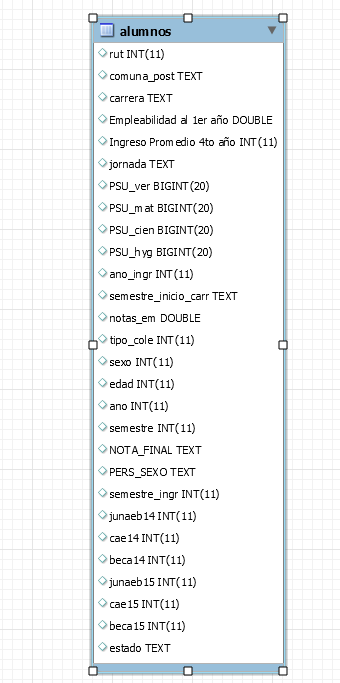
\includegraphics[width=8cm,height=8cm] {areastaging.png} 
	\caption[Tabla resultante]{Tabla resultante}
	\label{fig:bdarea}
\end{figure}

Los datos procesados se pueden apreciar en la Figura \ref{fig:bdarea}, la cual tiene principalmente variables de la ``Institución y Carrera'' y del ``Desempeño del Alumno'' definidas en la tabla de los constructos, Tabla \ref{tabla:Tablou de variables}, desestimando las variables de ``Motivaciones del Alumno'', debido a que no existe información de dichas variables en los datos proporcionados, por lo que para efecto de este estudio, se propone un mecanismo para capturar estos datos, y solo procesar modelos con la data existente.\\

El mecanismo a proponer es generar encuestas a final de cada semestre que capte y actualice las variables correspondientes a las motivaciones del alumno, de tal modo poder analizar la situación del alumno de manera semestral.\\


\subsection{Muestra de Datos}

La muestra de datos está configurada por 756 registros, de los cuales 743 pertenece a alumnos activos y 13 pertenece a alumnos que han abandonado la carrera.\\

La muestra de datos presenta un desbalanceo en las clases, esto ocurre precisamente cuando existen un conjunto muy pequeño pero significativo de datos, como es para este caso la clase abandono. Para corregir este problema se utilizarán diferentes operadores en la muestra con la herramienta \textit{RapidMiner}, de manera de balancear los datos.  


\subsection{Variables}

A continuación, se muestra una tabla con variable para modelar los datos de los dos conjuntos, el conjunto de jornada de vespertina no se consideran los puntajes PSU debido a que la institución tiene otro mecanismo de ingreso y la mayoría de las observaciones tiene esos campos vacíos.\\

\begin{longtable}{| p{3cm}| p{2cm} | p{7cm} |}
			\hline
			Variable & Tipo & Descripción \\
			\hline \hline
			\endfirsthead
			
			\hline
            Variable & Tipo & Descripción \\
            \hline \hline
            \endhead
            Rut & N/A & Identificador	\\ \hline			
			Comuna & N/A & Nombre de las comunas de residencia\\ \hline
			Genero & Discreto & Toma los siguientes valores, Femenino = 1; Masculino=2; F=1\\ \hline
			Edad & Continuo & Se considera edad del año 2014\\ \hline
			Tipo establecimiento de origen & Discreto & Toma los siguientes valores, Municipal=1; Particular Subvencionado=2; Particular Pagado =3;\\ \hline
			Notas enseñanza media & Continuo & Rango entre 10 y 70\\ \hline
			PSU lenguaje matemáticas & Continuo & Rango de 150 a 850\\ \hline
			PSU matemáticas & Continuo & Rango de 150 a 850\\ \hline
			PSU ciencias & Continuo & Rango de 150 a 850\\ \hline				
			Acreditación Institucional & Discreto & Toma los siguientes valores,  No Acreditada=0; Acreditada=1\\ \hline
			Carrera & N/A & Nombre de carrera\\ \hline
			Jornada & Discreto & Toma los siguientes valores,  Diurna y Vespertina\\ \hline
			Empleabilidad al 1er año & Continuo & Rango en porcentaje 0 a 100\\ \hline
			Ingreso promedio 4to año & Continuo & Rango en dinero\\ \hline
			Carrera acreditada & Discreto & Toma los siguientes valores,  No Acreditada=0; Acreditado=1\\ \hline 
			Promedio notas acumuladas & Continuo & Rango entre 10 y 70 \\ \hline
			Beca14 & Discreto & Toma los siguientes valores,  No Beca=0; beca=1\\ \hline
			Beca15 & Discreto & Toma los siguientes valores,  No Beca=0; beca=1\\ \hline
			Junaeb14 & Discreto & Toma los siguientes valores,  No Junaeb=0; Junaeb=1\\ \hline
			Junaeb15 & Discreto & Toma los siguientes valores,  No Junaeb=0; Junaeb=1\\ \hline
			Cae14 & Discreto  & Toma los siguientes valores,  No Cae=0; Cae=1 \\ \hline
			Cae15 & Discreto & Toma los siguientes valores,  No Cae=0; Cae=1\\ \hline
			Estado & Discreto & Toma los siguientes valores,  Activo y Abandono\\ \hline
			 \hline
		\caption{Variables.}
		\label{tabla:variablesdiurna}
\end{longtable}	



En las tablas anteriormente presentadas, se definió dos tipos de variables \cite{variables}:

\begin{itemize}
	\item Variables Discretas: Son variables que toma un conjunto de valores determinados, es decir, no acepta cualquier valor, solo los que existen el en conjunto, por ejemplo, Genero toma dos valores, Masculino y Femenino.
	\item Variables Continuas: Son variables que pueden tomar un valor fijo dentro de un intervalo, por ejemplo, los puntajes PSU puede tomar cualquier valor dentro del rango 150 a 850.
\end{itemize} 





\subsection{Procesos en RapidMiner}

La construcción de los modelos se implementó con la herramienta \textit{RapidMiner} utilizando como entrada las tablas generadas anteriormente.\\

\begin{figure}[H]
	\centering 
	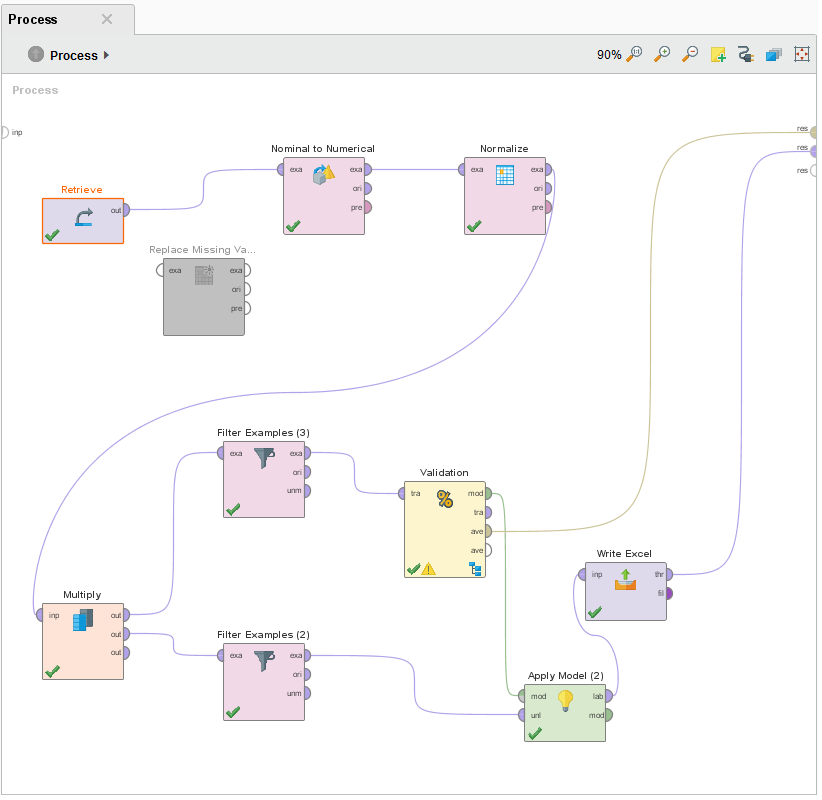
\includegraphics[width=12cm,height=7cm] {proceso.png} 
	\caption[Proceso de Predicción]{Proceso de Predicción}
	\label{fig:proceso}
\end{figure}

La herramienta \textit{RapidMiner} permite a través de operadores, construir un proceso. Los procesos son una serie de pasos constituidos por operadores. La Figura \ref{fig:proceso} representa el proceso construido para generar la predicción de los datos. La descripción de cada operador se detalla en el Anexo \ref{ch:anexo-b}\\

\begin{figure}[H]
	\centering 
	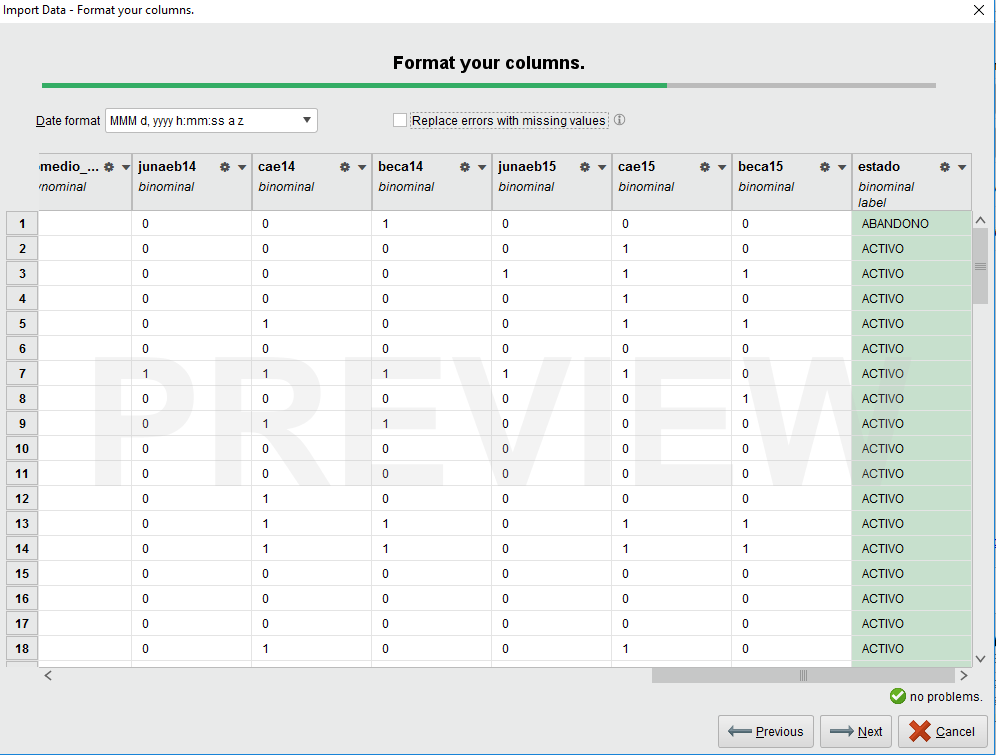
\includegraphics[width=12cm,height=7cm] {importdatos.png} 
	\caption[Importación de datos]{Importación de datos}
	\label{fig:importdata}
\end{figure}

El primer paso antes de operar el proceso construido, es importar los datos para entrenar y predecir. Las variables se definen como binominal para variables con dos tipos de datos y polinominal para variables con más de dos datos distintos, junto a ello se define el rol a cumplir dentro del modelo, para este caso, se tomó como rol identificador la variable ``rut'' y como rol etiqueta (variable a predecir) ``estado'', Figura \ref{fig:importdata}.

\begin{figure}[H]
	\centering 
	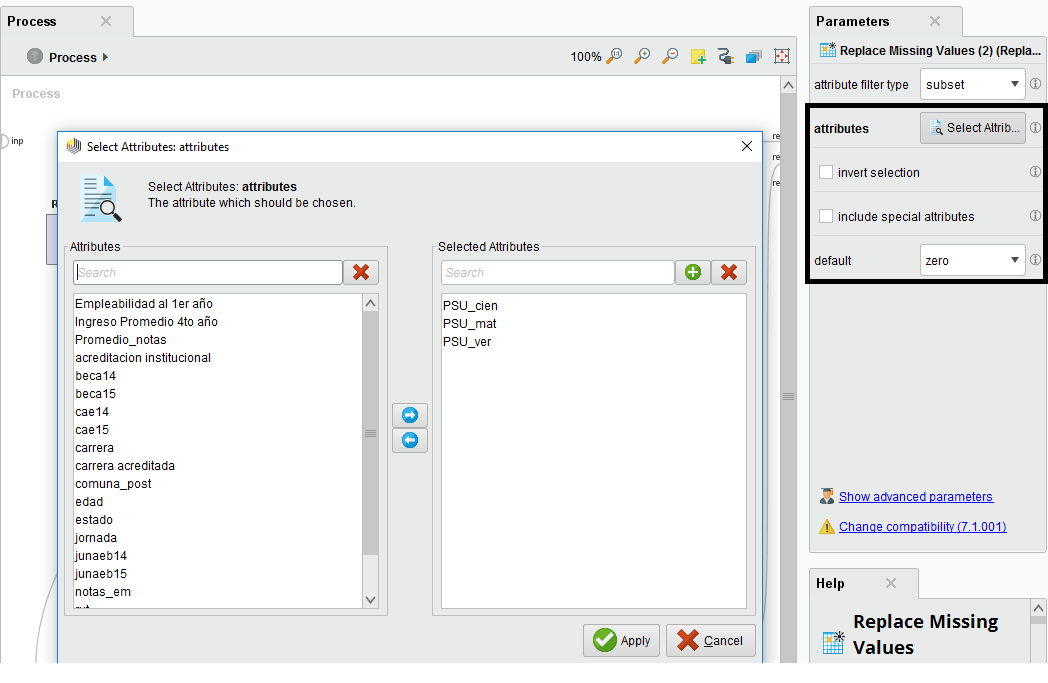
\includegraphics[width=12cm,height=7cm] {remplazodatos.png} 
	\caption[Remplazar de datos vacios]{Remplazar de datos vacíos}
	\label{fig:remplazadata}
\end{figure}

Los datos cargados son accedidos por el operador ``Retrieve'', luego pasa al operador  ``Replace Missing Values'' el cual reemplaza los valores vacíos de las variables seleccionadas, en este caso se seleccionaron las variables de ``PSU'' los cuales tienen datos vacíos, estos datos serán reemplazados por ceros como se puede ver en la Figura \ref{fig:remplazadata}.\\

Luego de que los datos son reemplazados, pasan al operador ``Nominal to Numerical'', el cual transforma todas las variables a numéricas, para luego pasar al operador ``Normalize'', normalizando los datos, luego al operador ``Weight by Chi Squared'' el cual ordena los datos por peso estadístico utilizando Chi Cuadrado, luego al operador ``Select by weights'' el cual selecciona las variables con el peso más alto del operador anterior, luego pasa al operador ``Multiply'' el cual multiplica los datos generando dos conjuntos, el primero para ser entrenado y el otro para validar, separados por los operadores ``Filter Example'', el conjunto a ser entrenado pasa hacia los operadores ``Sample (Bootstrapping)''y ``Sample'' los cuales balancean el conjunto de datos con el fin de disminuir el sesgo hacia una clase.\\


\begin{figure}[H]
	\centering 
	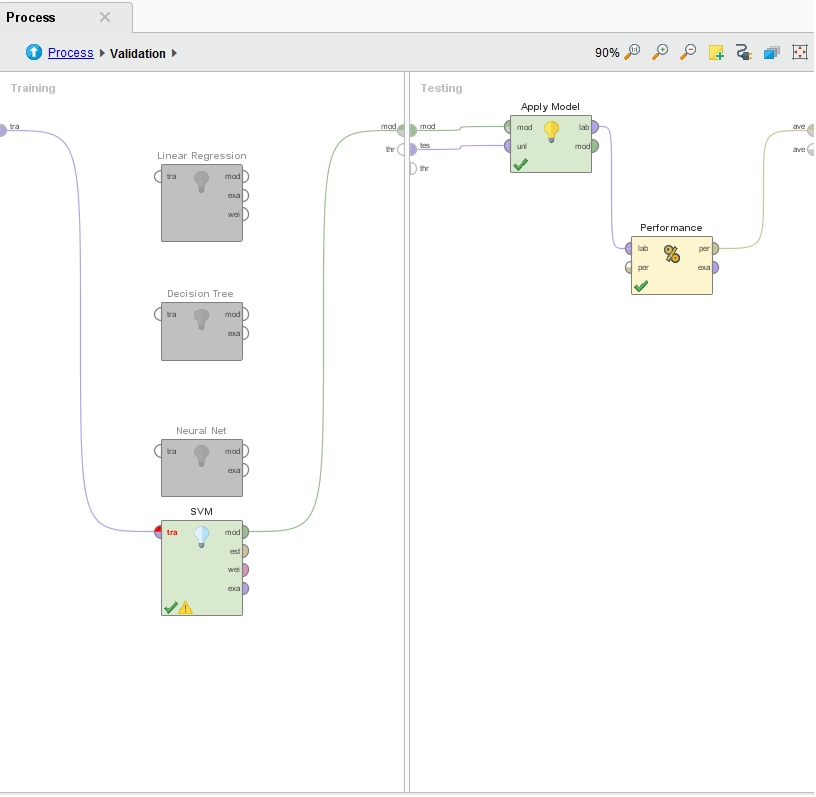
\includegraphics[width=12cm,height=7cm] {provalidacion.png} 
	\caption[Validación]{Validación}
	\label{fig:validacion}
\end{figure}

En el operador ``Validation'' se definen el porcentaje de datos a entrenar del total del conjunto de datos, en este caso se especifica un 70 \%. En este operador, se puede seleccionar los operadores de predicción, que para este estudio serán los cuatros que se muestran en la Figura \ref{fig:validacion}.

\section{Modelamiento}

El modelamiento se configuro de la siguiente manera, se replicaron 26 observaciones, 13 de abandono y 13 de activo, dejando la variable a predecir vacía de un total de 781 observaciones.\\

El detalle del resultado de las cuatro técnicas de predicción utilizadas en el conjunto de datos, se especifica la matriz de confusión.\\

La matriz de confusión es una herramienta que permite visualizar el desempeño de un algoritmo empleado para aprendizaje supervisado. Las columnas representan el número de predicciones por clases y las filas representan las instancias de la clase. Esta herramienta permite ver si el sistema está confundiendo dos clases \cite{matriz}.\\



\subsection{SVM}
	
\begin{figure}[H]
	\centering 
	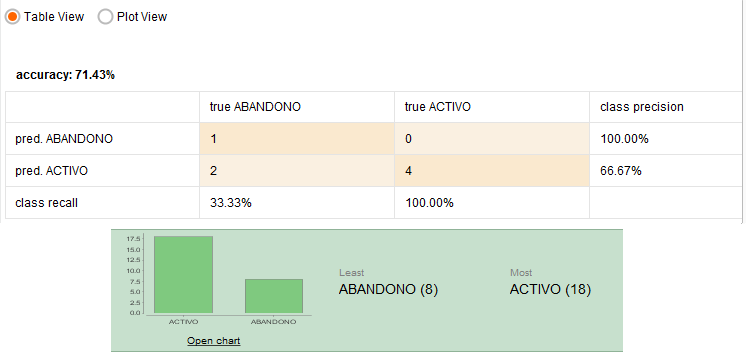
\includegraphics[width=10cm,height=3cm] {svndiurno.png} 
	\caption[Matriz de Confusión SVM]{Matriz de Confusión SVM}
	\label{fig:svndiurno}
\end{figure}	
	
La matriz de confusión que se muestra en la Figura \ref{fig:svndiurno} indica que SVM obtuvo una precisión del 71.43\%, especificando que la clase ACTIVO tuvo una precisión del 66.67\%, mientras que la clase ABANDONO tuvo 100\%.


\subsection{Regresión Lineal}
	
	\begin{figure}[H]
		\centering 
		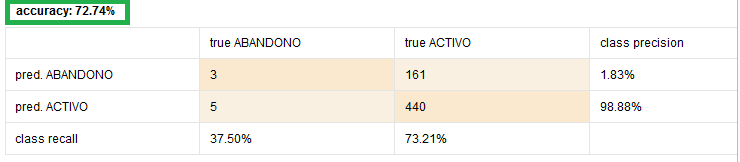
\includegraphics[width=10cm,height=3cm] {rldiurno.png} 
		\caption[Matriz de Confusión Regresión Lineal ]{Matriz de Confusión Regresión Lineal }
		\label{fig:rldiurno}
	\end{figure}	
	
	La matriz de confusión que se muestra en la Figura \ref{fig:rldiurno} indica que Regresión Lineal obtuvo una precisión del 85.71\%, especificando que la clase ACTIVO tuvo una precisión del 80\%, mientras que la clase ABANDONO tuvo 100\%. 
		



\subsection{Red Neuronal}
	
	\begin{figure}[H]
		\centering 
		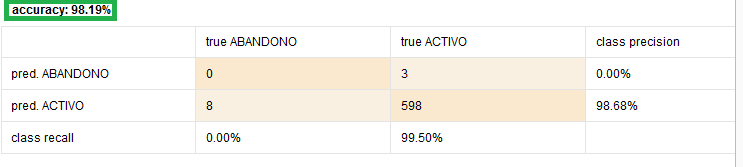
\includegraphics[width=10cm,height=3cm] {rndiurno.png} 
		\caption[Matriz de Confusión Red Neuronal ]{Matriz de Confusión Red Neuronal }
		\label{fig:rndiurno}
	\end{figure}	
	
	La matriz de confusión que se muestra en la Figura \ref{fig:rndiurno} indica que Red Neuronal obtuvo una precisión del 85.71\%, especificando que la clase ACTIVO tuvo una precisión del 80\%, mientras que la clase ABANDONO tuvo 100\%. 
	


\subsection{Árbol de Decisión}
	
	\begin{figure}[H]
		\centering 
		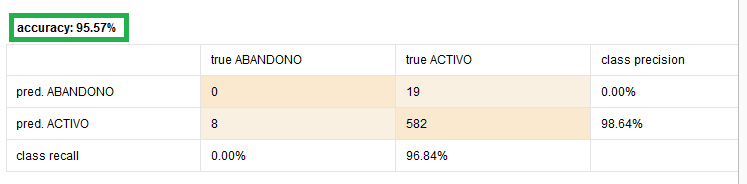
\includegraphics[width=10cm,height=3cm] {addiurna.png} 
		\caption[Matriz de Confusión Árbol de Decisión ]{Matriz de Confusión Árbol de Decisión}
		\label{fig:addiurna}
	\end{figure}	
	
	La matriz de confusión que se muestra en la Figura \ref{fig:addiurna} indica que Árbol de Decisión obtuvo una precisión del 85.71\%, especificando que la clase ACTIVO tuvo una precisión del 100\%, mientras que la clase ABANDONO tuvo 75\%.
	

	

\section{Resultados}

Dentro de los resultados obtenidos en los algoritmos de predicción probados, se comportan de manera muy similar, con diferencias muy pequeñas en las predicciones de cada clase, los algoritmos de Regresión Lineal, Red Neuronal y Árbol de Decisión obtuvieron una precisión del 85.71\%, mientras que SVM tuvo una precisión más baja, un 71.43\%. \\


En general los tres de los cuatro algoritmos tienen desempeños muy similares en la predicción, con diferencias mínimas en su precisión, sin embargo, las predicciones dependen mucho de los datos entrenados. Los resultados que se presentaron fueron con una muestra balanceada (la misma cantidad de clases) por ende es más preciso que otro resultado.\\

